\section{Problem 4-1 Power laws}

Consider the degree distribution functions $p_k$ of the following two undirected networks:

\begin{figure}[h]
	\centering
	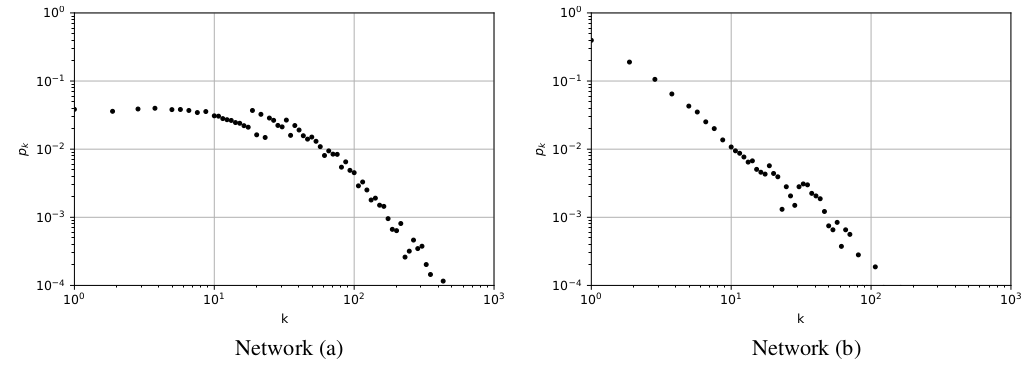
\includegraphics[width=0.9\linewidth]{images/problem41_degree_distribution_networks.png}
	\caption{A simple graph with 4 connected triples.}
	\label{distribution}
\end{figure}

\begin{enumerate}
	\item One of these networks is approximately scale-free, the other is not. Identify the scale-free network and explain how you came to your conclusion.
	
	Network b is is scale free. 
	Figure \ref{distribution} shows the log-log plots of the degree distribution of the two networks a and b. For scale-free networks the degree distribution forms a straight line across the diagonal. This is given for network b.
	
	\item A particular network is believed to have a degree distribution that follows a power law. A random sample of nodes is taken and their degrees are measured. The degrees of the first twenty nodes with degrees 10 or greater are: 
	
	16  17  10  26  13  14  28  45  10  12
	12  10  136  16  25  36  12  14  22  10
	
	For $K_{min} = 10$, estimate the exponent $\gamma$ of the power law using the estimation method presented in the lecture.
	Hint: you only have to estimate the exponent (see Slide 4-33)!
	Calculate the error $\sigma$ of your estimation using the equation $\sigma = \frac{\gamma - 1}{\sqrt{N}}$
	
	\vspace{0,75cm}
	The following solution is based on Slide 4-28 Estimating the degree exponent. From step 1. (Estimate value of the degree exponent corresponding to $K_{min}$) following formula is used:
	
	\begin{equation}
	\gamma = 1 + N \biggl[ \sum_{i=0}^N (ln(\frac{k_i}{K_{min} - \frac{1}{2}})) \biggr]^{-1}
	\end{equation}
	
	Now the values $N=20$, $k_i$ from the list above and $K_{min} = 10$ are inserted:
	
	\begin{equation*}
	\gamma = 1 + 20 \biggl[ ln(\frac{16}{20-\frac{1}{2}}) + ln(\frac{17}{20-\frac{1}{2}}) + ln(...) + ... \biggr]^{-1}
	\end{equation*}
	
	\begin{equation*}
	\gamma \approx -14,17
	\end{equation*}
	
	Based on $N$ and $\gamma$ the error $\sigma$ is calculated:
	\begin{equation*}
	\sigma = \frac{\gamma - 1}{\sqrt{N}} = \frac{-14,17 - 1}{\sqrt{20}} = -3,39
	\end{equation*}
	

\end{enumerate}